\documentclass[10pt,aspectratio=169]{beamer}
\usetheme{Montpellier}
\usepackage{amsmath,amssymb,tikz}

\title{Geometry And Topology Talk}
\author{Speaker}
\date{\today}

\begin{document}
\begin{frame}\titlepage\end{frame}

\begin{frame}{Geometric Object}
  \begin{itemize}
    \item Space, manifold, complex, graph, or moduli object.
    \item Local model and global invariant.
    \item Orientation, metric, chart, or coefficient convention.
  \end{itemize}
\end{frame}

\begin{frame}{Guiding Diagram}
  \centering
  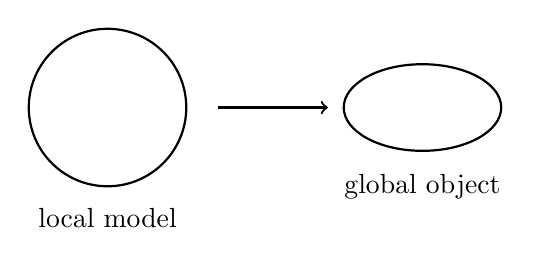
\begin{tikzpicture}[scale=1]
    \draw[thick] (0,0) circle (1);
    \draw[->,thick] (1.4,0) -- (2.8,0);
    \draw[thick] (4,0) ellipse (1 and .55);
    \node at (0,-1.4) {local model};
    \node at (4,-1.0) {global object};
  \end{tikzpicture}
\end{frame}

\begin{frame}{Main Invariant}
  \begin{block}{Invariant}
    Define the invariant and its normalization convention.
  \end{block}
  \begin{theorem}
    State how the invariant classifies, obstructs, or detects structure.
  \end{theorem}
\end{frame}

\begin{frame}{Examples And Non-Examples}
  Use examples to prevent definitions from becoming purely formal.
\end{frame}
\end{document}
